\documentclass[10pt,twocolumn,hidelinks,letterpaper]{article}

\usepackage[table]{xcolor}
\usepackage{cvpr}
\usepackage{times}
\usepackage{epsfig}
\usepackage{graphicx}
\usepackage{amsmath}
\usepackage{amssymb}

\usepackage[utf8x]{inputenc}
\usepackage[english]{babel}
\usepackage{url}
\usepackage{lipsum}

\usepackage[framed, numbered]{matlab-prettifier}
\usepackage{listings}
\usepackage{setspace}
\usepackage{color} %red, green, blue, yellow, cyan, magenta, black, white
\usepackage{geometry}
\usepackage{subcaption}
\usepackage{graphicx}
\usepackage{float}


% Include other packages here, before hyperref.

% If you comment hyperref and then uncomment it, you should delete
% egpaper.aux before re-running latex.  (Or just hit 'q' on the first latex
% run, let it finish, and you should be clear).
\usepackage[breaklinks=true,bookmarks=false]{hyperref}

\cvprfinalcopy % *** Uncomment this line for the final submission

\def\cvprPaperID{****} % *** Enter the CVPR Paper ID here
\def\httilde{\mbox{\tt\raisebox{-.5ex}{\symbol{126}}}}

% Pages are numbered in submission mode, and unnumbered in camera-ready
%\ifcvprfinal\pagestyle{empty}\fi
\setcounter{page}{1}
\begin{document}

%%%%%%%%% TITLE
\title{01TXFSM - Machine Learning and Deep Learning \\
\vspace{0.3in}
Final Project \\
First Person Action Recognition}

\author{
  Eros Fanì - s269781\\
  Politecnico di Torino\\
  {\tt\small eros.fani@studenti.polito.it}
  \and
  Gabriele Trivigno - s276807\\
  Politecnico di Torino\\
  {\tt\small gabriele.trivigno@studenti.polito.it}
  \and
  Cristiano Gerbino - s277058\\
  Politecnico di Torino\\
  {\tt\small s277058@studenti.polito.it}
}

\maketitle
%\thispagestyle{empty}

\lstset{language=python,%
  %basicstyle=\color{red},
  breaklines=true,%
  morekeywords={matlab2tikz},
  keywordstyle={\small \color{blue}},%
  morekeywords=[2]{1}, keywordstyle=[2]{\small \color{black}},
  identifierstyle={\small \color{black}},%
  stringstyle={\small \color{mylilas}},
  commentstyle={\small \color{mygreen}},%
  showstringspaces=false,%without this there will be a symbol in the places where there is a space
  numbers=left,%
  numberstyle={\small \color{black}},% size of the numbers
  numbersep=7pt, % this defines how far the numbers are from the text
  emph=[1]{error,warning},emphstyle=[1]{\small \color{red}} %some words to emphasise
  %emph=[2]{word1,word2}, emphstyle=[2]{style},
}

%%%%%%%%% BODY TEXT
\newcommand{\quotes}[1]{“#1”}
\newcommand{\reff}[1]{Figure \ref{#1}}
\setlength{\parindent}{0pt}
\setstretch{0.1}
\setlength{\parskip}{1em}
\definecolor{TopRow}{HTML}{E6E6FF}

\begin{abstract}


\end{abstract}

\section{Introduction}
The main scope of this project was the field of First Person Action Recognition, which is one of the up-and-coming domains in modern Computer Vision, due to the recent spread of wearable devices, often camera-equipped.
Even though action recognition and video analysis in general have been topics of research for quite some time now, this particular task introduces some newly faced challenges such as the strong egomotion component, which is inevitable as cameras are placed directly on the actor. Moreover the First Person point of view lacks some important information about the actor and its pose, showing only a part of the scenario, making inference harder. The most frequently adopted techniques to tackle this issues combine spatial information, taken from RGB frames, and motion clues, extracted in various ways, such as temporal stream networks based on optical flow, attention modules or 3D CNNs. We will discuss in depth some of this methodologies, highlighting in our opinion what are the weaknesses of such approaches, and proposing possible ways to circumvent them.

\subsection{Goals}
The first goal of the project was to replicate the main results of \cite{egornn}. Afterwards, we integrated the cited architecture with the self-supervised block proposed in \cite{sparnet}, implementing it in 2 different ways.

After trying to replicate these experiments with the hyperparameters setting reported in \cite{egornn}, with the experience acquired we chose other sets of hyperparameters that could potentially fit better our dataset of interest, and so performed a grid search upon them.

At last we have tried to improve the performances of the results of \cite{egornn} and \cite{sparnet} with some innovative ideas of our own.


\subsection{Our contribution}

\section{Related works}
Existing literature has underlined how the must crucial information to encode into features in order to obtain good performances on the task of First Person Action Recognition are the hands motion of the actor, and the appearance of objects manipulated, as well as their interaction. Putting together this 2 fundamental pieces of information is perhaps the most challenging task, and more importantly doing so without complicating too much the architecture, which could lead to high computational costs, cutting of potential on-line applications. \cite{egornn} proposes a spatial attention mechanism to focus on the region consisting of the object, arguing that objects handled are strongly representative of egocentric activities. To keep track of said objects throughout frames, this spatial attention is paired with a with a convLSTM module, whose purpose is to temporal encode the frame-level features formerly extracted. In addition to this, they also use a temporal network fed with optical flow images, following the purpose of better encoding motion changes in the considered videos. The task is then addressed with a late fusion of the 2 outputs with a dense layer to finally perform the classification step. Whilst reasonably successful, this approach consists of a two stream network, which requires several training stages
resulting in a massive number of parameters to train. \cite{sparnet} argues that adding a self-supervised block which leverages motion maps at the output of the CNN backbone can provide the convLSTM module with a richer input that already encloses motion information. They show that in this way the network is able to obtain a meaningful enough representation of both appearance and movement to achieve state-of-the-art results, so that the temporal network is no longer needed. Many other works recognize the importance of slimming the architecture to avoid having to train a 2 stream network. \cite{motfilt} introduces a unified model that aims at representing spatio-temporal relationship using only RGB frames, eliminating the heavy computation time required to extract optical flow, which makes the most difference at test time, once the model has been deployed. In their MFNet they insert motion filter blocks in the middle of CNN layers, that act upon feature maps extracted from shared-networks feed-forwarded by two consecutive input frames. The flow is estimated moving each channel of these feature maps in a 
different spatial direction $\delta := (\Delta x, \Delta y)$. \cite{reprflow}
argues that the procedure described, though advantageous parameter-wise and computation-wise, suffer from inferior performance compared with more powerful two-stream networks. They maintain such performance gap is due to the iterative optimization that standard optical flow methods implement and that \cite{motfilt} failes to reproduce. To overcome this issue they propose a new, fully-differentiable, layer, built to extract flow from any CNN feature map. By learning the flow parameters of a smaller resolution CNN tensor, in an end-to-end fashion together with the CNN training, they claim to
achieve the same representational power as traditional flow methods, and even better since flows optimized for activity recognition is different from true optical flow.
This last two works introduce a great way to encode motion clues in the features extracted, but none of them combine this information with a temporal representation of those features. Whereas \cite{egornn} fails to exploit RGB frames to get motion informations beyond appearances. Even though \cite{sparnet} tries to overcome this with the motion segmentation task, we found that their approach can sometimes lacks of precision in identifying the region of interest, since it acts on very high-level features.
In this project we propose three new different approaches. First of all, we use an improved version of the self-supervised block adopted in \cite{sparnet}to integrate in the work of \cite{egornn}, eliminating the need of a second network and improving the granularity of the motion encoding using higher resolution maps matched with lower level features. Afterwards we adopt the representation-flow layer proposed by \cite{reprflow} together with a temporal encoding module to better exploit temporal relationships in the features extracted. Finally we experimented with a different approach: encoding the concept of dynamics directly into the convLSTM module, adding a discriminator classifier that has been trained to discern whether it has been fed with static frames, or actual video frames. 

\subsection{Data exploration}

The dataset under analysis is a modified version of GTEA61\footnote{Georgia Tech Egocentric Activity Datasets: \small{\url{http://cbs.ic.gatech.edu/fpv/}}}. The dataset contains the videos in form of frames, and also two kind of preprocessed images: \textit{motion maps} and \textit{optical flows}. The folder schema of the dataset is shown in \reff{folder_schema}. Videos represent 61 class actions performed by 4 different users (\textit{S1}, \textit{S2}, \textit{S3}, \textit{S4}). Sometimes for some actions more than one video is available. The total number of videos in the dataset is, however, 457, which actually means that it is a quite small dataset.

\begin{figure*}
	\centering
	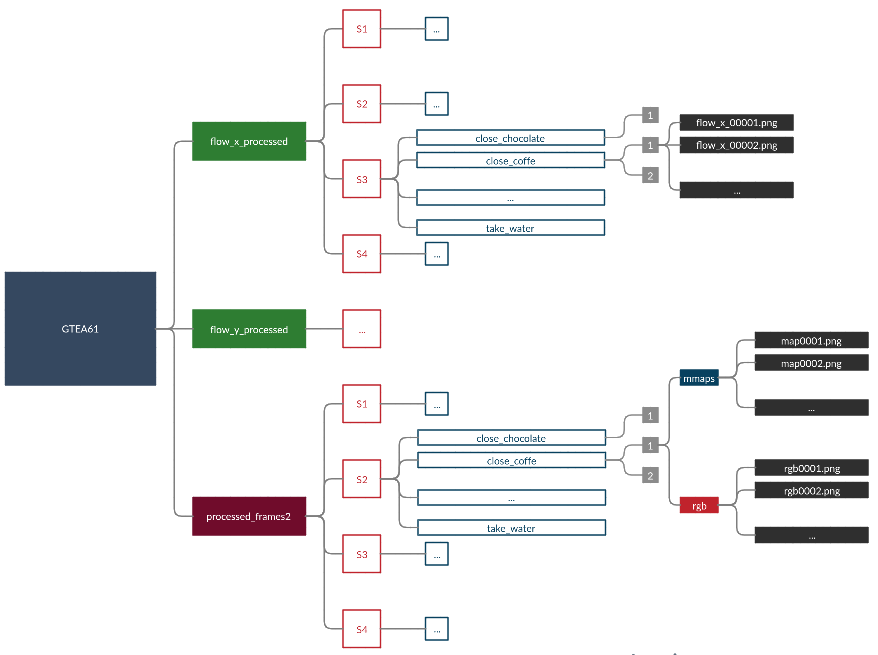
\includegraphics[width=.9\linewidth]{images/folder_schema.png}
	\caption{Folder schema of our GTEA61}
	\label{folder_schema}
\end{figure*}

The optical flow methods try to calculate the motion between two image frames which are taken at times $t$ and $t + \Delta t$ at every voxel position. The warp flow methods try also to remove the motion of the wearable camera. We have two kind of these last representations in our dataset: one computed in the horizontal axis (folder \textit{flow\_x\_processed}) and one other computed in the vertical axis (folder \textit{flow\_y\_processed}).

The motion maps are special black-and-white images which represent the spatial location in which the Motion Segmentation task of \cite{sparnet} focuses its attention per each frame. The mmaps present large similarities with the warp flows.

The differences between the kind of available images in our dataset are shown in \reff{image_comparison}.

\begin{figure*}
  \centering
  \begin{subfigure}{.24\linewidth}
  	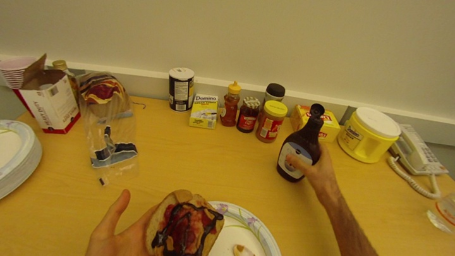
\includegraphics[width=\linewidth]{images/img_comp/rgb0001.png}
  \end{subfigure}
  \begin{subfigure}{.24\linewidth}
  	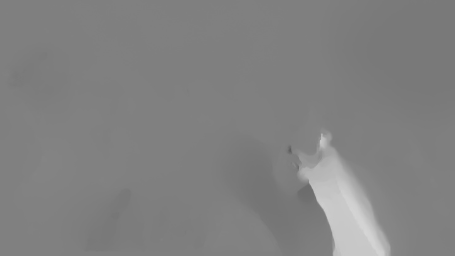
\includegraphics[width=\linewidth]{images/img_comp/flow_x_00002.png}
  \end{subfigure}
  \begin{subfigure}{.24\linewidth}
  	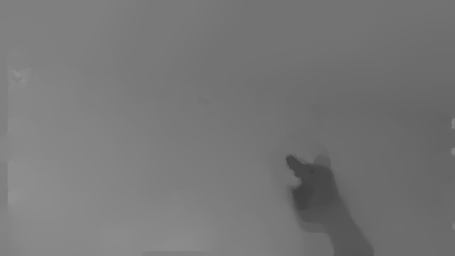
\includegraphics[width=\linewidth]{images/img_comp/flow_y_00001.png}
  \end{subfigure}
  \begin{subfigure}{.24\linewidth}
  	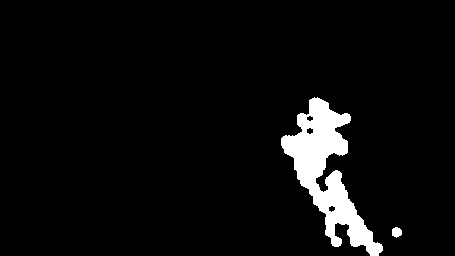
\includegraphics[width=\linewidth]{images/img_comp/map0001.png}
  \end{subfigure}
  \begin{subfigure}{.24\linewidth}
  	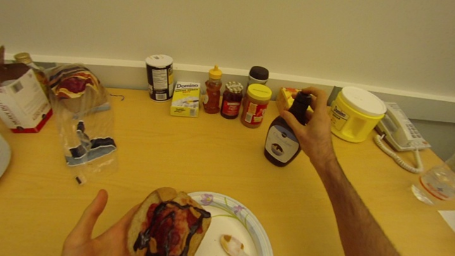
\includegraphics[width=\linewidth]{images/img_comp/rgb0011.png}
  \end{subfigure}
  \begin{subfigure}{.24\linewidth}
  	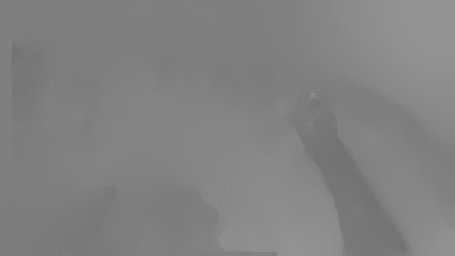
\includegraphics[width=\linewidth]{images/img_comp/flow_x_00011.png}
  \end{subfigure}
  \begin{subfigure}{.24\linewidth}
  	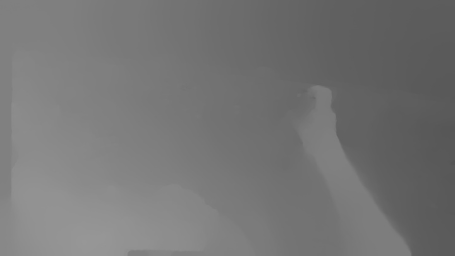
\includegraphics[width=\linewidth]{images/img_comp/flow_y_00011.png}
  \end{subfigure}
  \begin{subfigure}{.24\linewidth}
  	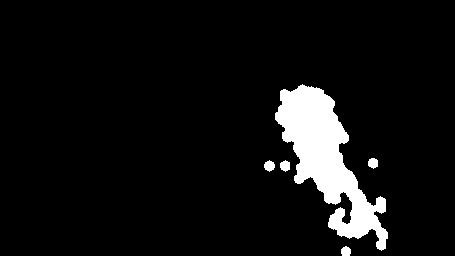
\includegraphics[width=\linewidth]{images/img_comp/map0011.png}
  \end{subfigure}
  \begin{subfigure}{.24\linewidth}
  	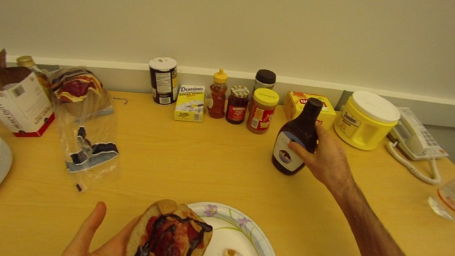
\includegraphics[width=\linewidth]{images/img_comp/rgb0020.png}
  \end{subfigure}
  \begin{subfigure}{.24\linewidth}
  	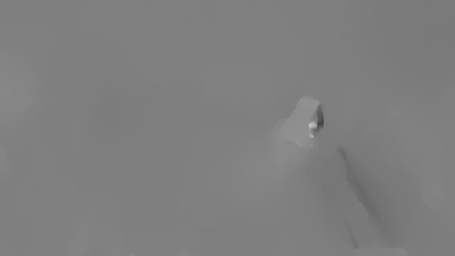
\includegraphics[width=\linewidth]{images/img_comp/flow_x_00020.png}
  \end{subfigure}
  \begin{subfigure}{.24\linewidth}
  	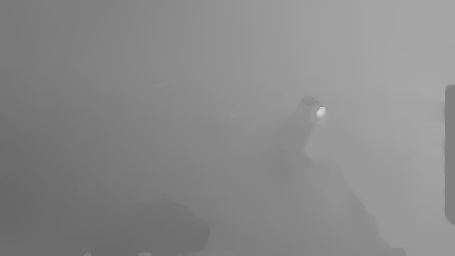
\includegraphics[width=\linewidth]{images/img_comp/flow_y_00020.png}
  \end{subfigure}
  \begin{subfigure}{.24\linewidth}
  	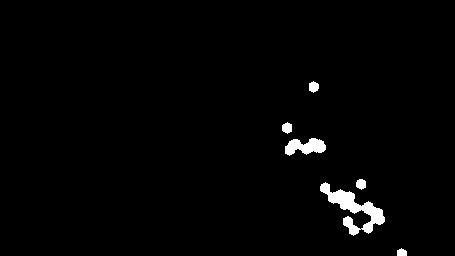
\includegraphics[width=\linewidth]{images/img_comp/map0020.png}
  \end{subfigure}
  \caption{Types of images in our dataset. In this example is shown a sample of images from the \textit{close\_chocolate} action. From the left column to the right column: rgbs, warp flows x, warp flows y, motion maps}
  \label{image_comparison}
\end{figure*}

\subsection{Data cleaning}

The dataset was almost clean already from the beginning, but we encountered two problems within it:
\begin{itemize}
  \item there were hidden useless folders \textit{.DSstore} inside each one of the user folders. These have been removed
  \item some of the first mmaps of some videos were missing. In these cases we have simply duplicated the second mmap
\end{itemize}

\section{Descriptions of the models}

Here we describe the models that we have used to perform our experiments.

\subsection{Egornn}

\textit{Egornn} is a Recurrent Neural Network. The overall architecture of \textit{Egornn} is shown in \reff{egornn_arch}. This net is based on \textit{resnet34}\cite{resnet}, which constitutes the main block. \textit{resnet34} has five convolutional layers inside itself: with respect to \reff{egornn_arch} they are: \textit{Conv}, \textit{Layer1}, \textit{Layer2}, \textit{Layer3} and , \textit{Layer4}. From now on we will refer to these blocks respectively \textit{conv1}, \textit{conv2}, \textit{conv3}, \textit{conv4} and \textit{conv5}.

At the termination of the \textit{resnet34} is placed a \textit{Spatial Attention Layer}. It calculates a \textit{Class Activation Map} (CAM) that is capable to identify the image regions that have been used by the CNN to identify the class under analysis. It is computed by taking the output of the \textit{softmax} layer and the output of \textit{conv5} and taking the linear combination of all the weights of \textit{conv5} and the weights of the softmax.

% We can graphically see some of our CAMs in \reff{cams}.
%%% ADD CAMS %%%

The output of the CAM is then sent to a \textit{softmax} layer to obtain a probability map, which is called \textit{Spatial Attention Layer} (SAM). The output of the SAM is finally multiplied, cell by cell (Hadamard product), with the output of \textit{conv5}, obtaining another tensor of weights which is sent to a \textit{Convolutional Long Term Support Memory} block (ConvLSTM).

The reason for the usage of the ConvLSTM block is that, up to now, what the net does is to take each frame and to try to make predictions based only on the features that the net can extract from those frames, without taking into consideration the temporal encoding of frame level features. The convLSTM block take into consideration, for each frame $i$, both the output of the SAM for the layer i and the output of the ConvLSTM for the layer $i-1$, constituting a recursive structure.

The last output of the ConvLSTM (the output obtained from the last frame of a particular video) is average pooled and reshaped to obtain a final classification layer with 61 neurons (i.e. the number of classes of our dataset).

\begin{figure*}
	\centering
	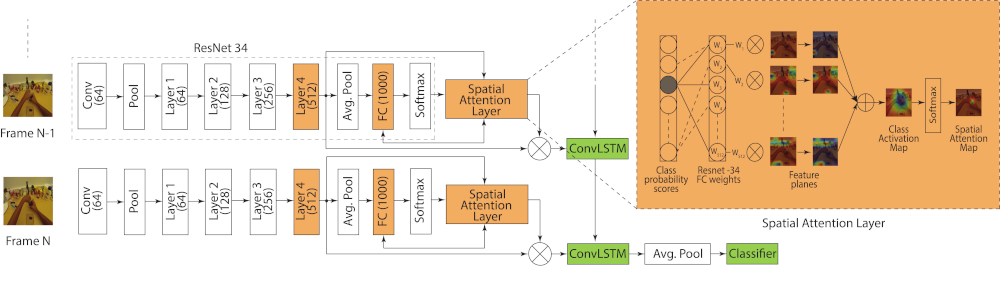
\includegraphics[width=\linewidth]{images/egornn.png}
	\caption{Architecture of \textit{egornn}}
	\label{egornn_arch}
\end{figure*}

\subsection{Flow\_resnet34}

\textit{Flow\_resnet34} is just a \textit{resnet34} edited to work with the warp flows. It gets five warp flows from \textit{processed\_frames\_x} and five from \textit{processed\_frames\_y} in form of a tensor of ten channels and tries to make predictions on the 61 classes.

\subsection{Two stream model}

\textit{Egornn} learns appearence features, while \textit{flow\_resnet34} learns motion features. The way to join the two nets is to concatenate the two output layers and to add at the end a fully connected layer to get the class category scores.

\subsection{Motion Segmentation branch applied to egornn}

The problem which \cite{sparnet} tries to overcome is that in the two stream model motion and appearence are actually separately learned, without taking into account the spatial-temporal relationships.

We have built an architecture similar to \textit{sparnet}, where the \textit{motion segmentation block} is the same but the \textit{action recognition block} has been substituted by \textit{egornn} (like in one of the attempts in \cite{sparnet}). The architecture is shown in \reff{msblock_arch}. We have used this architecture with some granular variations during our experiments, but the main blocks are always as shown in \reff{msblock_arch}. The input of the convolutional layer of MS Block is taken from one of the convolutional layers of \textit{resnet34} of egornn (the actual layer varies with our experiments). Then, after the convolutional layer, there is a fully connected layer followed by a softmax which normalizes the weights between 0 and 1. \textit{mmaps ground truth} and \textit{rgb ground truth} represent the mmaps and the rgb after the trasformations. The trasformations applied to the mmaps are the same applied to the rgbs, plus a small amount of proper mmaps trasformations which always ends with a trasformation which linearizes the pixels (from a 2 dimensional tensor per mmap we get a 1 dimensional tensor per mmap). For the msblock these linearized pixels represent a real ground truth, because each of the output neurons of the MS Block is used to predict the values of the mmaps ground truth. The pixel losses are summed together (obtaining as result $L_{ms}$) and then are summed again with the \textit{egornn} loss ($L_c$). The final loss is used to compute the gradients to update the weights.

\begin{figure*}
	\centering
	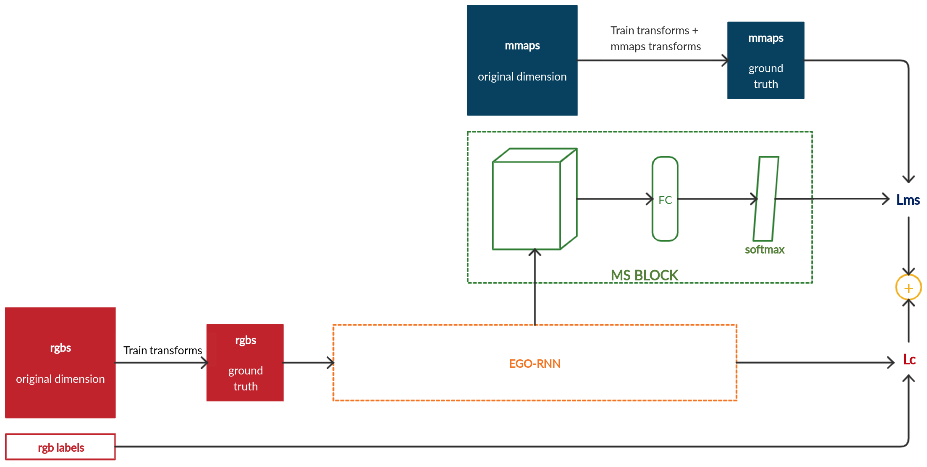
\includegraphics[width=\linewidth]{images/egornn+msblock_architecture.png}
	\caption{Generic architecture of motion segmentation branch applied to \textit{egornn}}
	\label{msblock_arch}
\end{figure*}

\subsection{Static-dynamic discriminator}

Starting from the model described above, we have added a final binary classifier to \textit{egornn} after the convLSTM, parallel to the other classifier already present which still tries to predict the actual class of the video. The idea was to force the net to learn the motion features from the rgbs. During the training phase this classifier gets 2 kind of sequences of frames: one is the same of the original classifier, while the other gets a sequence of identical frames. This discriminator should be able to recognize the actual videos from the static frames. In this way the gradients should adapt to focus the attention on the motion.

\section{Experiments}

Our nets are always trained on a predefined train set, which includes all and only the videos of the users \textit{S1}, \textit{S3} and \textit{S4}, while validation and test sets coincide and is constituted by all and only the videos of a single user, \textit{S2}. In addition, the weights of the \textit{resnet34} are pretrained on ImageNet. Each model is always validated while it is trained, so for each training phase we selected the weights with the highest accuracy at a particular epoch as the best ones.

Due to Colab limitations of GPU memory, we have only been able to perform experiments on a limited amount of frames (7 or, in less cases, 16). Due to this problem our results should be interpreted not as absolute value of the accuracy, but as a sort of relative value with respect to the number of frames for each video in our batches.

The size of our batches has always been left to 32, as well as the number of hidden units of the convLSTM module, fixed at 512. Our optimization algorithm is always Adaptive moment estimation (ADAM) with the only exception of \textit{flow\_resnet34}, for which it is Stochastic Gradient Descent (SGD). When using this last optimizer, the momentum has always been left to 0.9. The scheduler is a MultiStepLR scheduler, which decreases the original learing rate LR by a factor GAMMA at each value of STEP\_SIZE.

\subsection{Egornn}

We have replied some of the same experiments of \cite{egornn} on the original egornn. We have run each of these experiments three times and then we have averaged the results.

First, we have performed the classification by using the \textit{egornn} without and with the CAM. The training phase has been divided in two parts, as in the original paper:

\begin{enumerate}
  \item train of ConvLSTM and Classifier (green blocks in \reff{egornn_arch})
  \item train of conv5 (layer4 of \textit{resnet34}), FC(1000), Spatial Attention Layer (orange blocks in \reff{egornn_arch}) in addition to the previously listed blocks
\end{enumerate}

The values of the hyperparameters for the first stage are:

\begin{center}
	\setstretch{1}
  \scalebox{0.7}{
  	\begin{tabular}{|c|c|}
  		 \hline
  		 \textbf{LR} & 1e-3 \\
  		 \hline
  		 \textbf{WEIGHT\_DECAY} & 4e-5 \\
  		 \hline
  		 \textbf{NUM\_EPOCHS} & 200 \\
  		 \hline
  		 \textbf{STEP\_SIZE} & [25, 75, 150] \\
  		 \hline
  		 \textbf{GAMMA} & 0.1 \\
  		 \hline
  	\end{tabular}
  }
	\setstretch{0.1}
\end{center}

While, for the second stage, they are:

\begin{center}
	\setstretch{1}
  \scalebox{0.7}{
  	\begin{tabular}{|c|c|}
  		 \hline
  		 \textbf{LR} & 1e-4 \\
  		 \hline
  		 \textbf{WEIGHT\_DECAY} & 4e-5 \\
  		 \hline
  		 \textbf{NUM\_EPOCHS} & 150 \\
  		 \hline
  		 \textbf{STEP\_SIZE} & [25, 75] \\
  		 \hline
  		 \textbf{GAMMA} & 0.1 \\
  		 \hline
  	\end{tabular}
  }
	\setstretch{0.1}
\end{center}

Then, we have also trained \textit{flow\_resnet34} alone. In this case we used only 5 frames per each flow (x and y) due to the fact that for some videos no more than 5 frames were provided.

The values of the hyperparameters in this case are:

\begin{center}
	\setstretch{1}
  \scalebox{0.7}{
  	\begin{tabular}{|c|c|}
  		 \hline
  		 \textbf{LR} & 1e-2 \\
  		 \hline
  		 \textbf{WEIGHT\_DECAY} & 5e-4 \\
  		 \hline
  		 \textbf{NUM\_EPOCHS} & 750 \\
  		 \hline
  		 \textbf{STEP\_SIZE} & [150, 300, 500] \\
  		 \hline
  		 \textbf{GAMMA} & 0.5 \\
  		 \hline
  	\end{tabular}
  }
	\setstretch{0.1}
\end{center}

At last we performed the two stream training with the following values for the hyperparameters:

\begin{center}
	\setstretch{1}
  \scalebox{0.7}{
  	\begin{tabular}{|c|c|}
  		 \hline
  		 \textbf{LR} & 1e-2 \\
   		 \hline
   		 \textbf{LR\_FLOW} & 1e-4 \\
  		 \hline
  		 \textbf{WEIGHT\_DECAY} & 5e-4 \\
  		 \hline
  		 \textbf{NUM\_EPOCHS} & 250 \\
  		 \hline
  		 \textbf{STEP\_SIZE} & [1] \\
  		 \hline
  		 \textbf{GAMMA} & 0.99 \\
  		 \hline
  	\end{tabular}
  }
	\setstretch{0.1}
\end{center}

Where LR is the learning rate of \textit{egornn} and LR\_FLOW is the learning rate of \textit{flow\_resnet34}.

The summary of our results is shown in \reff{step1_table}.  From here it raises that the best model is the two-stream (joint train) with 16 frames, followed by EGO-RNN - stage 2 with 16 frames, which is behind the two-stream model by less than 1 point of mean accuracy. Due to the averaging between three identical runs we can rely on this result and assert that the contribution of \textit{flow\_resnet34} slightly increases the performances, but also that the most of the contribution is given by \textit{egornn}.

\begin{figure}[t]
	\centering
	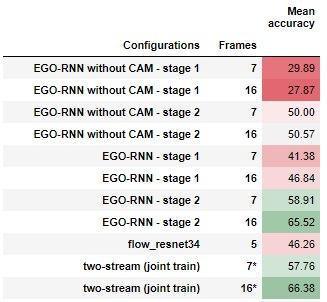
\includegraphics[width=\linewidth]{images/step1_table.jpg}
	\caption{Summary of the results over different configurations. Each value of the mean accuracy is the mean of the accuracies over three identical experiments. \small{*the number of frames refers to the \textit{egornn} branch (for the flow\_resnet34 branch the number of frames is always 5)}}
	\label{step1_table}
\end{figure}

In \reff{step1_acc} and \reff{step1_loss} are shown respectively the validation accuracy and the validation loss by epoch of one random extracted run per each one of the attempts with 16 frames (5 in case of \textit{flow\_resnet34}) and only for the stage 2 when a two stage training is requiered.

\begin{figure}[t]
	\centering
	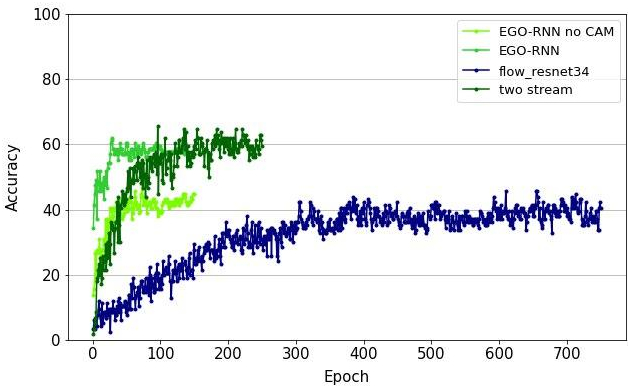
\includegraphics[width=\linewidth]{images/step1_acc.jpg}
	\caption{Validation accuracy by epoch of one random extracted run for the four most interesting training configurations}
	\label{step1_acc}
\end{figure}

\begin{figure}[t]
	\centering
	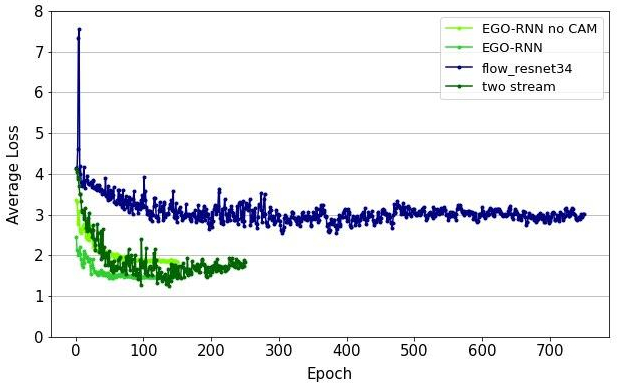
\includegraphics[width=\linewidth]{images/step1_loss.jpg}
	\caption{Validation loss by epoch of one random extracted run for the four most interesting training configurations. The losses are the average of each batch loss within a single epoch}
	\label{step1_loss}
\end{figure}

From \reff{step1_acc} and \reff{step1_loss} is even more evident that \textit{flow\_resnet34} is highly inefficient alone, and that the results with the CAM are heavily better than the results without the CAM (higher accuracy and lower loss at every epoch). The two-stream model requieres more time to get high accuracies, and overall it seems to have the same behaviour of \textit{egornn} when at full capacity, but it is noisier and so it is easier that for some epoch the accuracy is higher.

\subsection{Motion Segmentation branch applied to egornn}

First of all we have replied the same experiment of \cite{sparnet} (the one in which \textit{egornn} is the Action Recognition Block). The hyperparameters used are:

\begin{center}
	\setstretch{1}
  \scalebox{0.7}{
  	\begin{tabular}{|c|c|}
  		 \hline
  		 \textbf{LR} & 1e-3 \\
   		 \hline
  		 \textbf{WEIGHT\_DECAY} & 4e-5 \\
  		 \hline
  		 \textbf{NUM\_EPOCHS} & 150 \\
  		 \hline
  		 \textbf{STEP\_SIZE} & [50, 100] \\
  		 \hline
  		 \textbf{GAMMA} & 0.1 \\
  		 \hline
  	\end{tabular}
  }
	\setstretch{0.1}
\end{center}

for the stage1, while they are the following:

\begin{center}
	\setstretch{1}
  \scalebox{0.7}{
  	\begin{tabular}{|c|c|}
  		 \hline
  		 \textbf{LR} & 1e-4 \\
   		 \hline
  		 \textbf{WEIGHT\_DECAY} & 4e-5 \\
  		 \hline
  		 \textbf{NUM\_EPOCHS} & 150 \\
  		 \hline
  		 \textbf{STEP\_SIZE} & [25, 75] \\
  		 \hline
  		 \textbf{GAMMA} & 0.1 \\
  		 \hline
  	\end{tabular}
  }
	\setstretch{0.1}
\end{center}

for the stage2. We have decreased the number of epochs for the stage1 because we have observed that going too far with the epochs, with the loss decreased after the steps of the optimizer, would be meaningless and does not give any significant result.

The results with the same values for the hyperparameters are shown in \reff{ms_table}.

\begin{figure}[t]
	\centering
	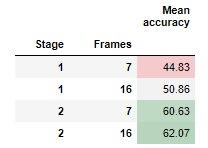
\includegraphics[width=.6\linewidth]{images/step2.1_table.jpg}
	\caption{Mean accuracies over three identical experiments with the same fixed set of values for the hyperparameters, by varying only the stage of training and the number of frames - classification experiment}
	\label{ms_table}
\end{figure}

As expected, the best performances are achieved after the second stage of training and with 16 frames.

We have also replied this experiment as a regression problem.
[REGRESSION IMPLEMENTATION]

In \reff{ms_reg_table} are shown the results.

\begin{figure}[t]
	\centering
	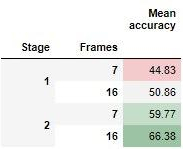
\includegraphics[width=.52\linewidth]{images/step2.3_table.jpg}
	\caption{Mean accuracies over three identical experiments with the same fixed set of values for the hyperparameters, by varying only the stage of training and the number of frames - regression experiment}
	\label{ms_reg_table}
\end{figure}

Also in this case the highest value of the accuracy is obtained for 16 frames. The first stage is exactly the same so we have not replied it three times more. For the second stage we observe that with this combination of values for the hyperparameters the regression performs more than 4 points better than classification with 16 frames, while the accuracies are roughly the same when the number of frames is 7.

We have performed also a complete grid search to improve the performances of the net.

Before starting, it has been execuded a brief tuning step for the stage 1 of training, which is the same for both the classification and the regression methodologies. The values of interest have been STEP\_SIZE and GAMMA only. From this we obtained that the optimal values for the stage1 are exaclty the same used in the previous experiment.

After this preliminary step, the complete grid search has been executed only on the stage 2, which is the most important one. The number of selected frames is 16, for which we have seen that the performances are better than for 7. We have reduced NUM\_EPOCHS to 100 to save computational time (in addition the highest accuracy is rarely obtained after epoch 100). For the classification strategy the results are shown in \reff{ms_grid}, while for the regression they are shown in \reff{ms_reg_grid}.

\begin{figure}[t]
	\centering
	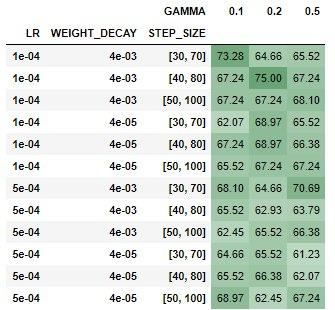
\includegraphics[width=\linewidth]{images/grid_no_reg_table.jpg}
	\caption{Accuracies at various combinations of hyperparameters for the classification strategy}
	\label{ms_grid}
\end{figure}

\begin{figure}[t]
	\centering
	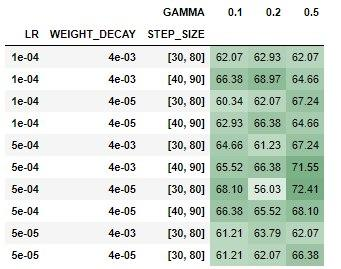
\includegraphics[width=\linewidth]{images/grid_reg_table.jpg}
	\caption{Accuracies at various combinations of hyperparameters for the regression strategy}
	\label{ms_reg_grid}
\end{figure}

As we can observe the best performances are achieved with:
\begin{itemize}
  \item $LR = 10^{-4}, WEIGHT\_DECAY = 4 \cdot 10^{-3}, STEP\_SIZE = [40, 80]$ for the classification method, for an accuracy of 75.00
    \item $LR = 5 \cdot 10^{-4}, WEIGHT\_DECAY = 4 \cdot 10^{-5}, STEP\_SIZE = [30, 80]$ for the regression method, for an accuracy of 72.41
\end{itemize}

In general we can say that the performances are better with the classification method, and this is a surprisingly result based on the observations without the grid. The reason for the previous result was that, as emerges from \reff{ms_grid} and \reff{ms_reg_grid}, the optimal values for the hyperparameters falls in a total different region with respect to the two different methodologies.

In \reff{grid_comparison} we can observe the effects of the values of the hyperparameters on the accuracy and on the loss of both train and validation and over three different experiments present in the grid search with the classification methodology. The colors of the graphs underline the different learning rate before ad after each step of the optimizer. The steps are shown on the x axis and marked with a vertical gray line. In (a) is shown the best result obtained, while (b) and (c) are representative examples with different tuned values for the hyperparameters. In (a) the loss already starts from a low value and the accuracy already starts from an high value.LR highly influences the starting point of the accuracy and the loss in epoch 1 (higher LR $\rightarrow$ lower initial accuracy and higher initial loss). To show this behaviour it has been picked the example in (b), which has the same STEP\_SIZE but different values for the other hyperparameters. We can observe that, from \reff{ms_grid}, there is not a tangible difference between the column with GAMMA = 0.1 and the column with GAMMA = 0.2, while it is more evident that with GAMMA = 0.5 the accuracy worsen a bit. So, it has been selected another example, (c),  with GAMMA = 0.1 (which is a different gamma with respect to (a)) and the same values of LR and WEIGHT\_DECAY (which differs from (a)), and with another STEP\_SIZE. The effect of this slight variation on the STEP\_SIZE seems to be not so meaningful, while the actual main characters of the different behaviour of the net are LR and WEIGHT\_DECAY, together with GAMMA which is good when it is 0.1 as well as when in is 0.2. As last observations:
\begin{itemize}
  \item is evident from all the three experiments that the train accuracy continue growing also when the validation accuracy starts flattening, and the behaviour is the relative one for the loss
  \item both the losses and the accuracies are \quotes{noisier} when the learning rate is higher
  \item the global behaviour is strongly influenced by the random batches which feed the net, and so the results should be intended within an error margin
\end{itemize}

\begin{figure*}
  \centering
  \captionsetup[subfigure]{justification=centering}
  \begin{subfigure}{.325\linewidth}
  	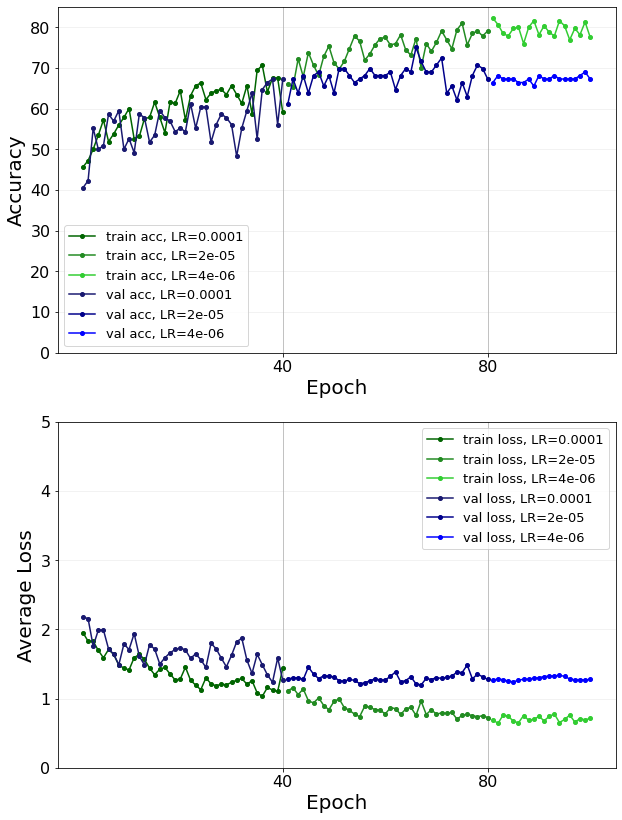
\includegraphics[width=\linewidth]{images/grid_comparison/acc75no_reg.png}
    \subcaption{\\LR = 1e-4\\WEIGHT\_DECAY = 4e-3\\STEP\_SIZE = [40, 80]\\GAMMA = 0.2\\Highest accuracy = 75.00\\at epoch 66}
  \end{subfigure}
  \begin{subfigure}{.325\linewidth}
  	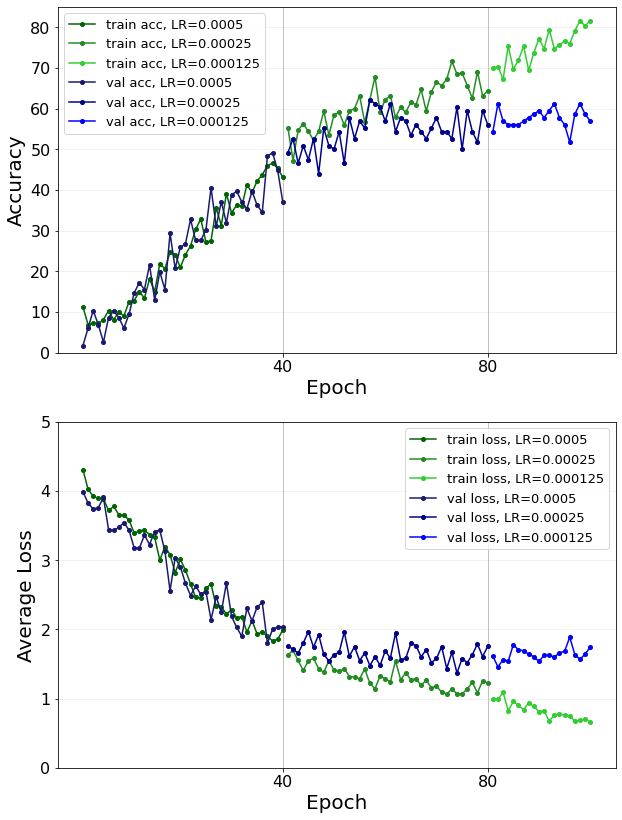
\includegraphics[width=\linewidth]{images/grid_comparison/acc62lr5e-4step4080gamma05_no_reg.png}
    \subcaption{\\LR = 5e-4\\WEIGHT\_DECAY = 4e-5\\STEP\_SIZE = [40, 80]\\GAMMA = 0.5\\Highest accuracy = 62.07\\at epoch 57}
  \end{subfigure}
  \begin{subfigure}{.325\linewidth}
  	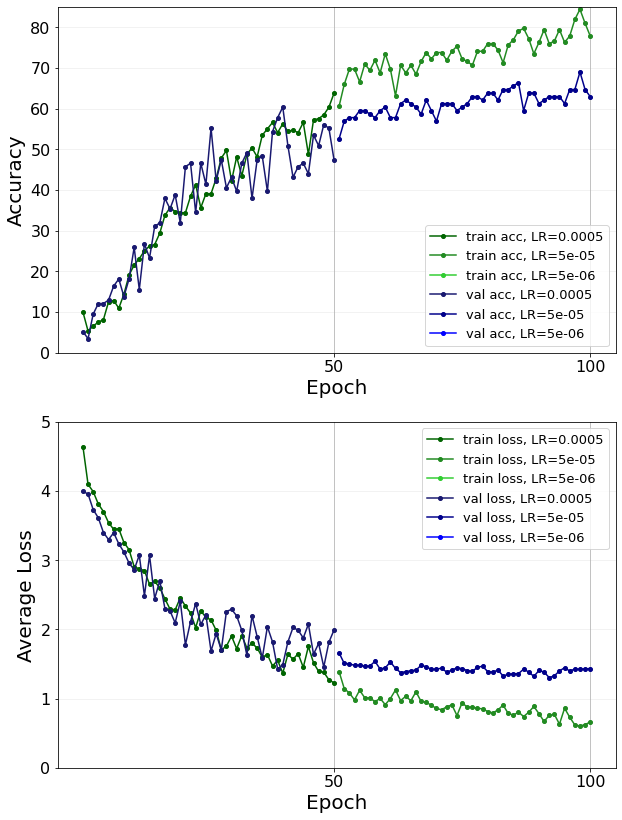
\includegraphics[width=\linewidth]{images/grid_comparison/acc69lr5e-4step50100gamma01_no_reg.png}
    \subcaption{\\LR = 5e-4\\WEIGHT\_DECAY = 4e-5\\STEP\_SIZE = [50, 100]\\GAMMA = 0.1\\Highest accuracy = 68.97\\at epoch 98}
  \end{subfigure}
  \caption{Comparison between three representative experiments in the grid search with the classification method}
  \label{grid_comparison}
\end{figure*}

To assert if there is an actual contribution of the Motion Segmentation branch and how much it is sgnificant we analyzed the loss on the mmaps with a special attention. Some examples of this loss are shown in \reff{loss_mmaps}.
%
% \begin{figure}[t]
%   \centering
%   \includegraphics{}
%   \caption{}
%   \label{}
% \end{figure}

As we can see from these graphs the loss on the train set stops to drop after a few bunch of epochs.

To overcome these problems we have tried to increase the resolution of the downsampled mmaps and to treat the problem as.

\begin{figure}[t]
	\centering

	\begin{subfigure}{.4\linewidth}
		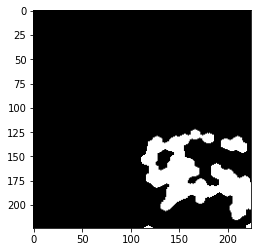
\includegraphics[width=\linewidth]{images/mmaps_example/downsampling224x224_bw.png}
	\end{subfigure}
  \begin{subfigure}{.57\linewidth}
    \begin{subfigure}{.32\linewidth}
  		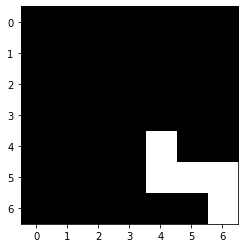
\includegraphics[width=\linewidth]{images/mmaps_example/downsampling7x7_bw.png}
  	\end{subfigure}
  	\begin{subfigure}{.32\linewidth}
  		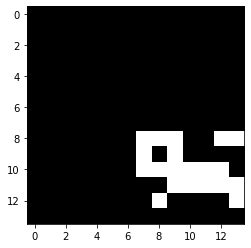
\includegraphics[width=\linewidth]{images/mmaps_example/downsampling14x14_bw.png}
  	\end{subfigure}
  	\begin{subfigure}{.32\linewidth}
  		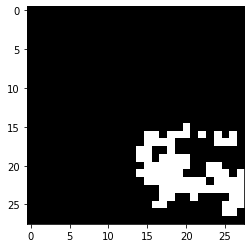
\includegraphics[width=\linewidth]{images/mmaps_example/downsampling28x28_bw.png}
  	\end{subfigure}
  	\begin{subfigure}{.32\linewidth}
  		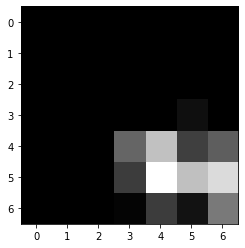
\includegraphics[width=\linewidth]{images/mmaps_example/downsampling7x7_gray.png}
  	\end{subfigure}
  	\begin{subfigure}{.32\linewidth}
  		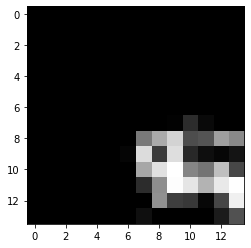
\includegraphics[width=\linewidth]{images/mmaps_example/downsampling14x14_gray.png}
  	\end{subfigure}
  	\begin{subfigure}{.32\linewidth}
  		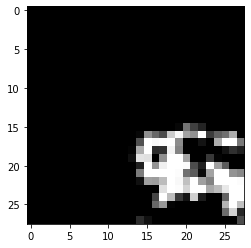
\includegraphics[width=\linewidth]{images/mmaps_example/downsampling28x28_gray.png}
  	\end{subfigure}
  \end{subfigure}

	\caption{}
	\label{mmaps}
\end{figure}

% In \reff{mmaps} we can observe an example of downsampled mmap at 7x7 resolution.




% \subsection



{\small
\bibliographystyle{ieee}
\bibliography{egbib}
}

\end{document}
